\setcounter{chapter}{8}
\setchapterabstract{This chapter delves into vertical agreements (VAs), which occur between firms operating at different levels of the supply chain (e.g., producers and retailers). While often less harmful to competition than horizontal agreements, VAs can still raise competition concerns if they lead to upstream or downstream foreclosure, facilitate collusion, or restrict intra- and inter-brand competition, particularly when market power is involved.
Types of restrictions include resale price maintenance (RPM), export bans, and exclusive territorial agreements, which can hinder market competition and innovation. However, beneficial effects such as mitigating the free-rider problem, enabling market entry, avoiding double marginalization, and resolving hold-up issues can balance restrictive outcomes.
Certain agreements, like selective distribution systems (SDA), are lawful if they meet qualitative criteria and are proportionate. SDAs are common in luxury or technically complex goods markets, helping preserve brand image and product quality. Restrictions on online sales are permissible if justified, proportionate, and uniformly applied, as seen in cases like Coty Germany. Lastly, EU law emphasizes balancing competitive harm against efficiency and pro-competitive benefits, using block exemptions and guidelines to assess agreements.}
\chapter{Vertical Agreements Analysis}
\vspace{-1.5cm}

{\chaptoc\noindent\begin{minipage}[inner sep=0,outer sep=0]{0.9\linewidth}\section{Vertical Arrangements}\end{minipage}}

    \Definition{
    Arrangements involving two (or more) independent firms operating at different levels of the production-distribution chain (producer, wholesaler, retailer). These agreements refer to the conditions under which the parties may purchase, sell or resell certain goods or services.
    }{Vertical Arrangement}

    Concluding a VA is always an option. A producer might deal with the final consumer directly, by vertical integration: Apple owns its brick \& mortar Apple stores and supplies many of its products on line through its e-shops “iTunes” and “App-Store” to costumers. In case of vertically integrated production, arrangements between undertakings at different levels of the supply chain are not caught by Article 101 (all the parties belong to the same single economic entity). (Apple also signed several vertical agreements with independent distributors)

    \Remark{
    Remember that agents and similar entities may be considered as part of the same entity when they do not bear any commercial/financial risk.
    }

\newpage
    Case law (in particular, ECJ in Allianz Hungaria):
    \begin{enumerate}
        \item Vertical agreements are often less damaging to competition than horizontal agreements (rationale: they do not imply a direct combination of market power). Many of them do not restrict competition at all (a purely qualitative selective distribution system; a non-exclusive distribution agreement).
        \item Usually---apart from restrictions by object (see point 4)---they are likely to raise competition concerns only where one or both the parties enjoy a high degree of market power in the upstream market, in the downstream market, or at both levels.
        \item There can be an anticompetitive effect at an \emph{interbrand} level (that is, possible harm to competitors of the parties upstream or downstream) or at an \emph{intrabrand} level (possible restriction of competition between retailers of the same brand).
        \item Some vertical restraints (RPM, export bans, and prohibition of passive sales) are considered by object restrictions.
    \end{enumerate}

    \subsection{Interbrand Effect}

        \begin{enumerate}
            \item \textbf{Upstream Foreclosure}: A Russian producer of crude oil, P1, signs an exclusive access and pumping contract with the owner of the TransEuropean crude oil pipeline D. D is a monopolist (there are no other pipelines connecting Russia to Western Europe). P2 and P3 are producers of crude oil, too.
        
            This VA has the effect of pushing P2 and P3 out of the Western European market for crude oil, unless they can immediately create their own pipelines D2 and D3.
        
            \item A similar foreclosure effect \textbf{Downstream} can be shown where there is only one producer and many distributors. An exclusive agreement may force all the competing distribution chains to exit the market\sn{\Note{Again, distributors may have an option of beginning production upstream.}}.
        
            \item In some circumstances, VA may also have the effect of \textbf{Softening Competition} upstream or downstream, facilitating collusion.
        \end{enumerate}

        Several parallel agreements on \emph{minimum resale prices} may have the effect of facilitating collusion upstream, i.e., between the producers of a certain good, by impeding the distributors to reduce the sell-out price.
        
        In a cartel environment, all the parties involved must observe the agreement on a set price or market allocation. If distributors were free to set prices, offer discounts, or sell outside the assigned area, it would be impossible to keep the cartel alive (plus: think about monitoring: who is cheating? P or D?).

        \Example{
        A and B are two producers of mobile phones. Given the demand, they know that the price that maximizes profits is Pm. However, they do not sell directly to final consumers, but through networks of dozens of independent distributors. The only way to defend their collusive agreement is by imposing their distributors to sell at Pm.
        }

    \subsection{Intrabrand Effects}

        \begin{itemize}
            \item \textbf{Market Sharing:} Rossignol ski assigns to X, Q, and Z a certain area on an exclusive basis.

                This territorial exclusivity may be set at regional or at national level\sn{\Example{For example, Rossignol ski may require:
                \begin{itemize}
                    \item The Italian retailer X not to sell to customers living in France and Switzerland.
                    \item The Swiss retailer Q not to sell to customers living in Italy and France.
                \end{itemize}}}.
                
            \item \textbf{Sell Out Price Control:} Rossignol ski requires its national retailers X, Q, and Z not to sell the new Rossignol Radius 30 World Cup giant slalom skis at less than the recommended price of €1,400.

            Many other possible restrictions: no-compete clauses, minimum amount of promotional investments, investments in stocks, pre-sale, post-sale services, no cross-selling, no internet sales, etc.

            These restrictions are \emph{intrabrand}, i.e., they do not affect competitors of Rossignol or their retailers (Fischer, Atomic, Head, and their distributors remain free to sell skis at any price to anyone).
        \end{itemize}


        Usually Intra-brand restrictions are not relevant when there is strong inter-brand competition. In other words, a restriction of intra-brand competition is likely to raise concerns only where inter-brand competition is already weak (However, by object restrictions which are always forbidden)\sn{\Note{In fact, if there is a sufficient level of competitive pressure between different brands inside the same relevant market, a rational producer would never impose useless restrictive clauses to its distributors because they would be unprofitable.}}. 

        \Example{
        P, a small producer, tries to impose a minimum sell-out price to distributors, D1 and D2. D1 and D2 are not going to accept such clause because they know that they may need to move the price according to what their (stronger) competitors will do. If they are not able to decrease the price pursuant to a price decrease effected by a competitor (or a competitor’s distributor), than they will lose market shares and exit the market.
        }

        EU antitrust law has always to do with some other EU goals, like the "creation of an internal market".

        Thus, the Commission is very skeptical when confronted with intrabrand restrictions containing export bans (like in the recent case \emph{Intendo}, €168 million in fines) or absolute territorial protection even if the parties do not enjoy a high level of market power.
        
        \Remark{
        Usually, while a restriction on active sales outside the assigned territory is tolerated (otherwise, there would be no exclusivity at all), a restriction on passive sales is considered a by-object infringement (like export bans).
        }
        
        Furthermore, a couple of very simple points:
        
        \begin{enumerate}[label=(\alph*)]
            \item Exclusivity is generally more anti-competitive than non-exclusive arrangements;
            \item A combination of different vertical restraints may usually increase the overall anticompetitive effects (i.e., exclusive distribution, plus resale price recommendation; plus non-compete covenants, etc.);
            \item Negative effects arising from vertical restraints are reinforced when several suppliers and their respective buyers organize their trade in a similar way (cumulative effects).
        \end{enumerate}

\section{By Object Restrictions}

        \subsubsection{Export Bans are sometimes indirect}

            Direct export bans are prohibited by object, and USUALLY not permitted under Article 101(3). However, also indirect export bans or disincentives to export are prohibited. 

            \Example{
            ZANUSSI provided that its guarantees were available to consumers in a particular Member State only if they bought the product from a distributor in the same Member State. For durable goods this is really a very strong disincentive to purchase the same good abroad.
            }
            
\section{Resale Price Minimum}

            Imposition upon distributors and retailers of fixed or minimum resale prices is prohibited because these agreements restrict competition by object (thus no \emph{de minimis} exception; no block exemption). In fact, RPMs:
            
            \begin{itemize}
                \item May facilitate collusion between suppliers by enhancing price transparency on the market.
                \item By eliminating intra-brand price competition, facilitate collusion between distributors. Strong or well-organised distributors may be able to force or convince one or more suppliers to fix their resale price above the competitive level and thereby help them to reach or stabilize a collusive equilibrium\sn{\Note{The immediate effect of RPM will be that all or certain distributors are prevented from lowering their sales price for that particular brand.}}. 
                \item RPM may be implemented by a manufacturer with market power to foreclose smaller rivals. The increased margin that RPM may offer to the distributor may induce the latter 
                \begin{enumerate}[label=(\alph*)]
                    \item to favour the particular brand over rival brands when advising customers, even where such advice is not in the interest of these customers, or 
                    \item not to sell these rival brands at all (pharmacies prefer to sell branded products because these products are more expensive than generic ones and they earn more).
                \end{enumerate}
                \item RPM may reduce dynamism and innovation at the distribution level. By preventing price competition between different distributors, RPM may impede more efficient retailers from entering the market or acquiring sufficient scale with low prices.
            \end{itemize}

        \subsubsection{While RPMs are forbidden “recommended” and “maximum” RP are not by object restrictions}

            \begin{itemize}
                \item \textbf{Fixed RPM} = fixed sell-out price. You must sell at 10.
                \item \textbf{Recommended RPM} = According to my market enquiry, you should sell at 10 (being free to under/over price).
                \item \textbf{Maximum RPM} = You are free to sell at any price below 15.
            \end{itemize}

            \Remark{
            Recommended and maximum resale prices are \textbf{not hard core restrictions}, and are also covered by the Block Exemption Regulation provided that they do not amount to a fixed or minimum sale price as a result of pressure from, or incentives offered by, any of the parties.
            }

            This may happen, for example, when it is not genuinely possible for the reseller to lower that recommended price (ECJ, C-279/06, \emph{CEPSA}); or when the producer fixes the maximum level of discount the distributor can grant from a prescribed price level.

            \textbf{Pioneer}: Sell-out price was in theory only recommended. However, pricing behaviour of dealers and distributors was highly monitored in order to avoid the "perverse" effect due to the widespread use of the clause \emph{best price guaranteed}, which obliges all distributors to decrease the sell-out price whenever any of them lowers the price of a product. Thus, Pioneer threatened to reduce or cease the supply of goods to price cutters.

            \Example{
            \textbf{CD MUSIC DISTRIBUTION CHANNELS IN THE US.} \\ 
            The US music majors were worried by the very high level of competition in the retail channel. Music shops were selling music CDs at below-cost price due to strong competition at distribution level. Thus, music shops asked the Majors to lower their sell-in prices in order to allow the retailers to maintain a positive margin. \\
            The majors reacted to these requests by introducing a policy according to which they would grant rebates and above all the reimbursement of promotional costs only if the retailers would agree to sell at a Minimum Advertised sell-out Price (MAP policy). \\
            This policy ended the price war at the reseller level and allowed the majors to recreate a period of “quiet life equilibrium”. Even if MAPs are not RPM, they may be considered an indirect mean to obtain the same result.
            }

    \subsection{Beneficial effects}

        A lot of beneficial effects may balance the restrictive ones. Some examples:
        
        \begin{enumerate}[label=(\alph*)]
            \item \textbf{The free-rider problem.} Why do we need to assign to a distributor an area of exclusivity?
        
            Roski is the Italian distributor of Rossignol skis and ski-boots. Roski would like to boost its sales in Italy. Thus, it starts offering several pre-sale and post-sale services, and promoting the product in order to create interest in it and increase its demand. Mainly, it offers several free training days with the World Cup winner Federica Brignone; free professional advice on the "radius" of skis and the choice of ski-boots, etc.
        
            Should this retailer be prepared to make these marketing/promotional investments if it feared that other retailers could sell the same products without participating in the cost of promoting them? \textbf{NO!}
        
            Obviously, it would refrain from offering pre-sales services if customers could firstly enjoy the service and then buy the product at another cheaper shop or retailer.
        
            Thus, exclusive distribution agreements may be used to prevent the free-riding problem, providing a distributor the incentive to promote a product effectively, thereby increasing the degree of inter-brand competition.
        
            \item \textbf{Opening up and entering new markets (first-time investments to create the demand).} It may be necessary to protect the distributor from competition so that it can recoup its initial investment by temporarily charging a higher price.
        
            Paddy, a producer of padel rackets and balls, is willing to enter the Asian market, where this sport is not known at all. Paddy doesn’t know the market and doesn’t want to risk it by itself. It thus identifies TennisB, a local distributor who is already active in the neighboring market of sports equipment for tennis.
        
            TennisB may promote this new sport by creating interest and facilities for it (i.e., opening a number of padel courts around Asia, organizing events and tournaments with some Argentinian "padel stars," etc.).
        
            TennisB should thus invest millions of euros for several years before selling the first pair of padel shoes and rackets. And obviously, this activity is very risky.
        
            No rational distributor would engage in such activity without exclusivity protection for a couple of years. In fact, without the exclusivity protection, a free rider could exploit TennisB’s promotional efforts and then enter the market and "rip all the customers" by fixing a lower price.
        
            \item \textbf{The Hold-up Problem}
        
            The hold-up problem refers to a situation in which a supplier needs to make client-specific investments and will not commit to it until supply agreements have been concluded.
        
            In order to persuade the producer to make the investment, a long-term supply agreement will be required, so that it knows that it will be able to recoup its costs (e.g., I will build a power plant that produces energy fully absorbed by the demand of a steel production facility only after the reassurance by the owner of the steel production facility that it will sign with me a 15-year exclusive purchasing contract).
        
            In other contexts, think of the specific hold-up problem when know-how has to be temporarily transferred from the producer to the distributor.
        
            Without a non-compete provision on the recipient of the know-how to ensure that it is not used by competitors of the owner, no rational producer would ever enter into a vertical agreement.
        
            \item \textbf{Avoiding double marginalization.}
        
            The price behavior of the retailer can run against the interests of the producer and its customers. If the exclusive distributor sets the price at an excessive level (above the monopoly price), the distributor increases its revenues and profits per unit, but the producer will quickly lose market shares (either due to substitution or the income effect). Thus, fixing a maximum resale price may help the producer to keep its sales levels and profits, but at the same time, RPM may also benefit customers.

            \Example{
            In summer, absent maximum rpm, service stations– especially in touristic area– increase the sell out price of gasoline and diesel; here the distributor may be better off if it is able to hold back all the price increase; the producer instead will be worse off because of the likely reduction in total quantities, even if the demand for gasoline and diesel is quite rigid
            }
        
            Suppose that $U$ is a monopolist and intends to sell its products at the monopolist level $p_m$. $U$ has a sole distributor in Italy, $D$, that by definition has monopoly power in the Italian market.

            \begin{figure}[ht]
                \centering
                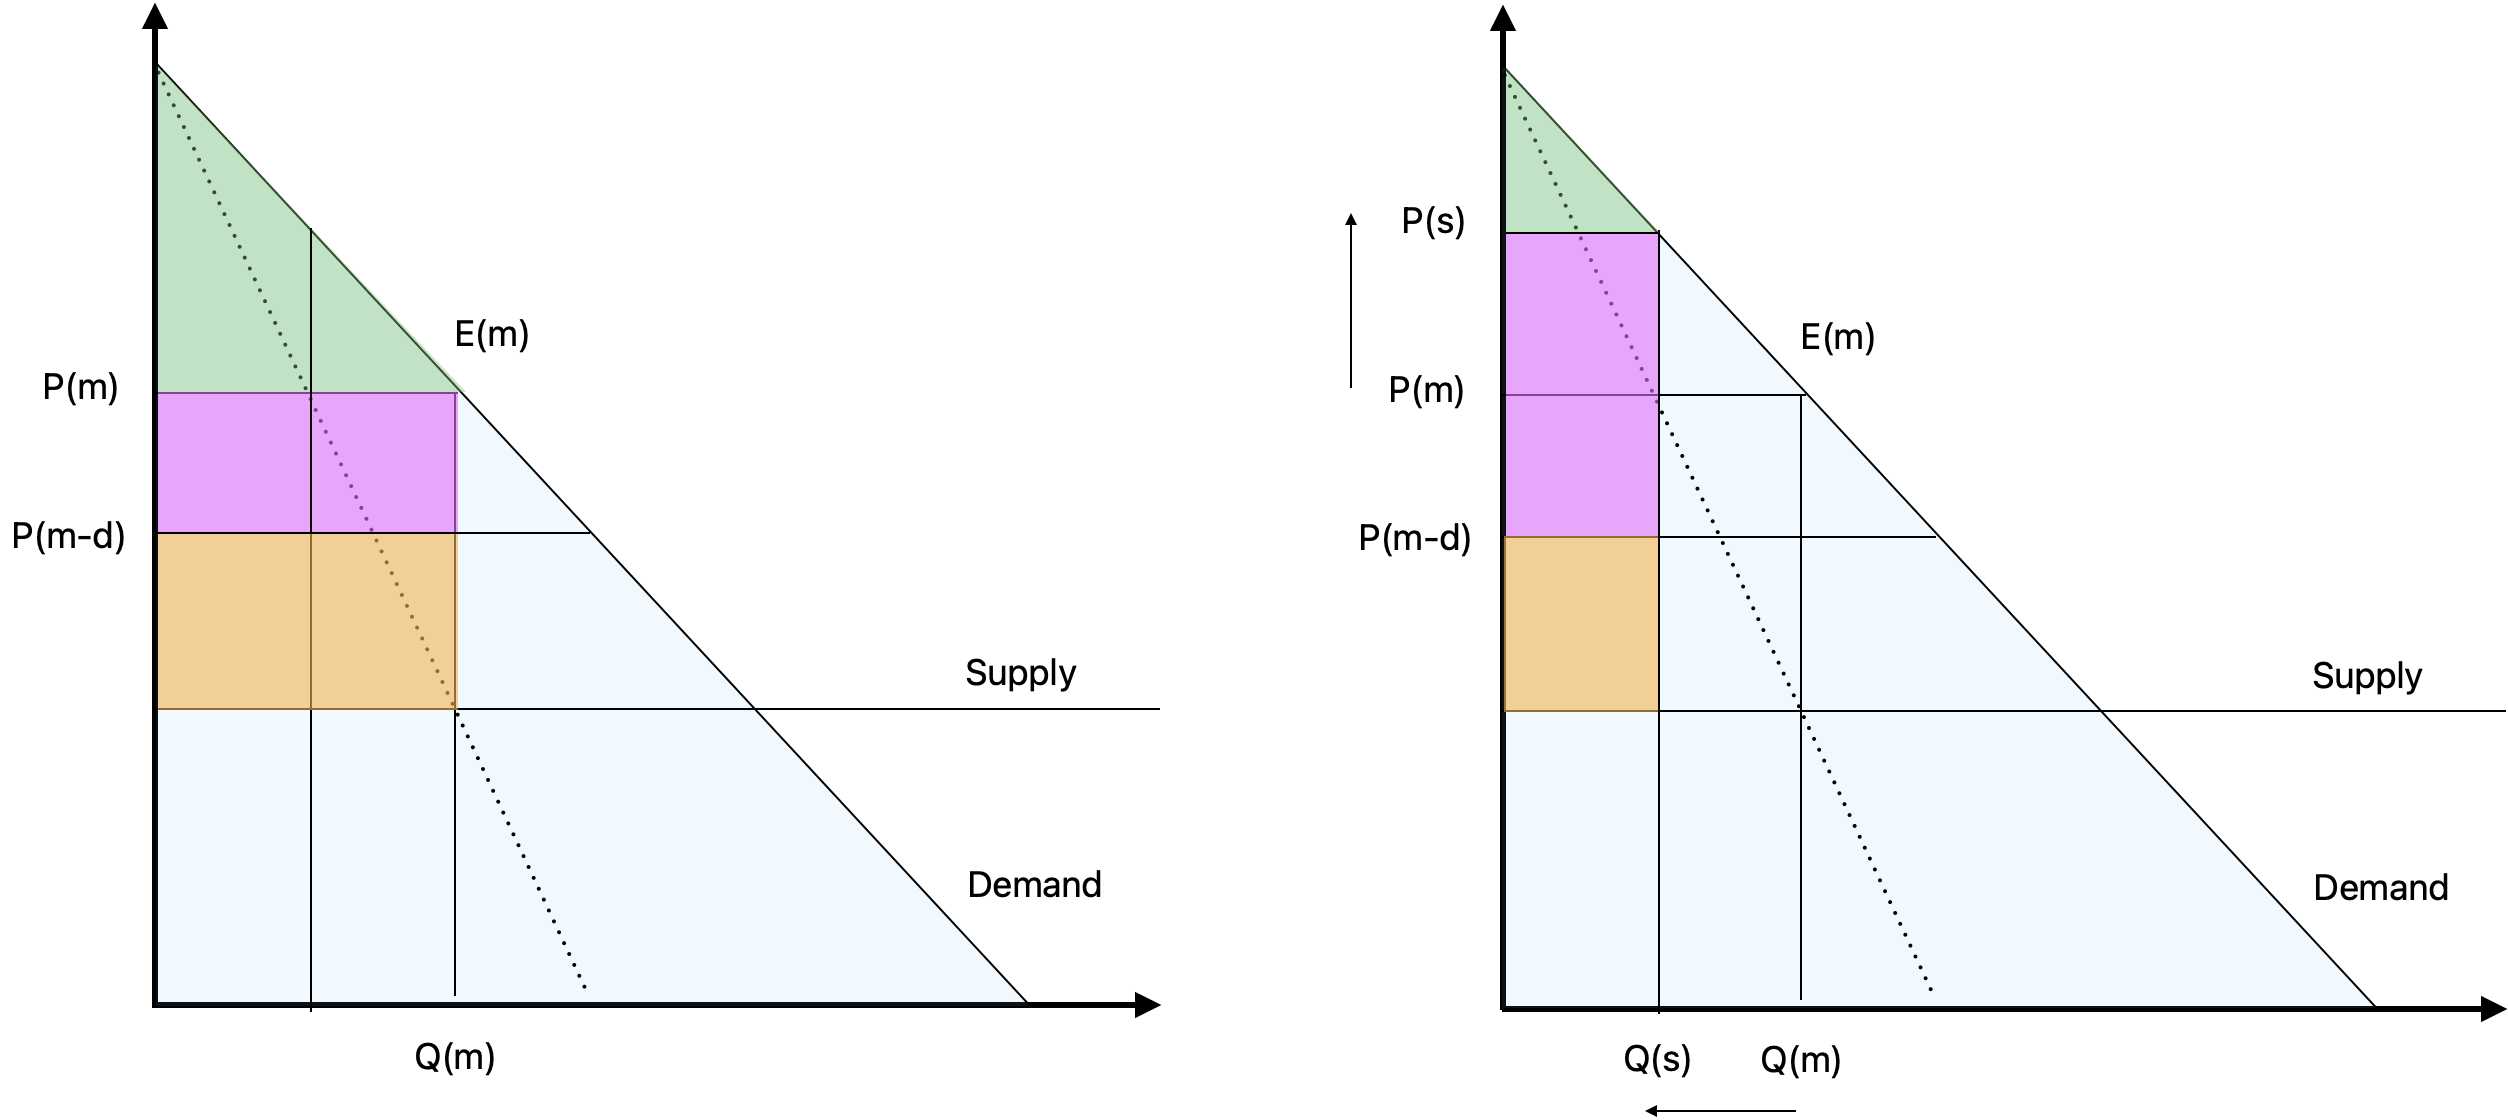
\includegraphics[width=1\linewidth]{double_marginalisation.png}
                \caption{D in purple, U in orange, Consumer surplus (CS) in green}
            \end{figure}
        
            $U$ sells its goods to $D$ at $p_{(m-d)}$ (the so-called sell-in price) because it recognizes a margin $d$ to $D$.
        
            However, given that $D$ has market power, it would desire to earn more than $d$, and begins to sell the product at a reselling price $p_s$ where $p_s > p_m$.
        
            In this scenario:
        
            \begin{itemize}
                \item $D$ may be better off (fewer sales but higher unit profits);
                \item $U$ is certainly worse off (fewer sales and thus less profits);
                \item At the societal level, given that $p_s$ is higher than $p_m$, not only will we have $\downarrow Q$ (decreased quantity) and $\uparrow P$ (increased price) and $\downarrow CS$ (decreased consumer surplus), but also a reduction of $PS$ (producer surplus) and a reduction of $TS$ (total surplus).
            \end{itemize}
        
            Thus, if $U$ is able to fix the maximum resale price (sell-out price) at $p_m$, it will maximize its profits and, at the same time, it will safeguard $TS$ (and $CS$, in comparison to the alternative scenario).
        
            In this specific case, fixing maximum resale prices has a positive effect on $TS$ and $CS$.
        \end{enumerate}


\newpage

\section{Appraisal of vertical agreements}

    \textbf{Two short cuts (safe harbor or safe haven):}
    
    \begin{itemize}
        \item \textbf{De minimis}: (except for by object restrictions, like export bans, RPM) a safe harbour is provided when upstream and downstream market shares are under the 15\% threshold.
        \item \textbf{Block Exemption Regulation}: If the agreement does not contain any "hardcore restrictions"---which are listed in Article 4 of the Regulation---then it must be considered lawful if the supplier’s and the buyer’s market share is below 30\%. Those hardcore restrictions mainly apply to intra-brand agreements and in particular:
        \begin{itemize}
            \item RPMs (maximum and/or recommended RPM are not prohibited);
            \item No absolute territorial restrictions (but a restriction on active sales is permitted).
        \end{itemize}
        Furthermore, even if not hardcore, other restrictions lead to non-application of the Regulation:
        \begin{itemize}
            \item Contract length exceeding 5 years;
            \item Other obligations concerning selective distribution systems.
        \end{itemize}
        \textbf{REMEMBER: What is not prohibited is permitted.}
    \end{itemize}
    
    In those cases, there is no need to make any balancing between procompetitive and anticompetitive effects: the former are automatically assumed to prevail over the latter.

    \Remark{
    If either market shares are larger than 30\% or the vertical agreement does not conform to the Block Exemption list of provisions, then the parties need to self-assess the agreement.
    }
    
    In doing so, they may refer to the case-law and the Vertical Guidelines which contain a detailed list of all the relevant factors that must be considered for the assessment.

\section{Exclusive distribution agreements}

    A supplier may grant exclusive distribution rights to a distributor for a particular territory.

    \Example{
    Barilla might appoint $X$ as its exclusive distributor for France and $Y$ as its exclusive distributor for Germany.
    Barilla may also agree not to sell its products directly in Germany and France.
    }
    
    \subsubsection{Most important antitrust concerns:}
    
    \begin{enumerate}[label=\alph*.]
        \item \textbf{Intrabrand competition will be reduced} (inside the same area/country): When you assign to each distributor a specified territorial area and impose a prohibition on active/passive sales outside the area, you confer upon them a monopoly in the assigned areas. This market partitioning may be dangerous when the market power of the supplier is strong because the distributor is not constrained by producers and/or distributors of other brands.
    
        \item \textbf{Market partitioning} (at national level): Exclusive Distribution Agreements (EDA) can divide national markets, especially when active and passive sales are forbidden by contract; passive sale prohibitions are a \emph{by object} restriction.
    
        \item \textbf{The use of exclusive distribution agreements may soften competition upstream and favor collusion.} Intrabrand restriction pushing an interbrand restriction.
    
        \item \textbf{Exclusive distribution may lead to foreclosure of other distributors }and thereby may reduce competition at that level (only when the distributor has very strong buyer power and there are barriers to entry at the downstream level).
    \end{enumerate}

    \Remark{
    A no active sales prohibition may be accepted; a no-passive sales prohibition is \textbf{strictly forbidden}
    }

    \subsubsection{Passive vs. active selling}
    
        \textbf{Passive selling} means responding to unsolicited requests from individual customers, including delivery of goods or services to such customers, "outside the assigned territory".
        
        For example, I’m the only Italian distributor of Rossignol Skis. I have been assigned the Italian territory. However:
        
        \begin{enumerate}[label=\alph*.]
            \item A French client comes to my firm’s premises and would like to buy 2 pairs of skis. This is a passive (unsolicited) sale that I should remain free to perform.
            \item The same applies if the French customer orders me by email one pair of skis (provided that I did not solicit him by, for example, direct ads or ads specifically tailored for French potential clients).
        \end{enumerate}
        
        \medskip

\noindent
        \textbf{Active selling} means actively promoting/advertising products outside the assigned territory. Obviously, if active selling was to be permitted by contract, the same concept of exclusive distribution should not exist.
        
        \Remark{
        From an antitrust standpoint, while a distribution agreement may contain a clause prohibiting active selling, passive selling cannot be limited; in that event, the agreement should be considered prohibited according to Article 101.
        }
        
    \subsubsection{EDA and the Internet}

        \textbf{In principle}, every distributor must be allowed to use the internet to sell its products; according to EU antitrust rules, the use of a website to sell products amounts to \emph{passive selling}.
        
        If an Italian customer visits the website of a Danish distributor and if such contact leads to a sale, that is treated as a passive sale.
        
        \medskip

\noindent
        Thus, we should label "hardcore" or \emph{by object} a restriction according to which:
        
        \begin{itemize}
            \item A distributor in one territory will prevent customers in another distributor’s territory from viewing its website or will automatically re-route customers to other distributors’ websites;
            \item A distributor will terminate customers’ transactions over the internet if their credit card data reveal an address that is not within the distributor’s territory;
            \item A distributor will limit its proportion of overall sales made over the internet;
            \item The distributor will have to pay a higher price for products intended to be resold online rather than offline.
        \end{itemize}


\section{Selective Distribution Agreements}

    Selective Distribution Agreements (SDA) are used by producers of:
    
    \begin{itemize}
        \item Branded products (luxury, cosmetics, perfumes);
        \item Products that need significant pre- and post-sales services;
        \item Products that are technically complex (e.g., cars, cameras, consumer durables, clocks, computers, etc.).
    \end{itemize}
    
    These products can be bought and resold only by authorized distributors and retailers. Thus, non-authorized distributors and retailers are excluded from the market.
    
    \Remark{
    SDA are used to keep the value of trademarks (e.g., \emph{“brand image”}: watches, cosmetics, jewelry) or the quality of the services connected to the product.
    }
    
    A selective distribution system is \textbf{not anti-competitive IFF:}
    
    \begin{itemize}
        \item The nature of the product justifies restricting the kind of outlets by which they may be resold; \textbf{AND}
        \item The criteria by which a supplier selects retail outlets through which its products are resold \textbf{ARE:}
        \begin{itemize}
            \item Purely qualitative in nature,
            \item Laid down uniformly for \textbf{ALL} potential retailers, and
            \item Applied in a non-discriminatory manner (e.g., suitably trained staff; suitable premises in an appropriate area; shop name; obligation to provide proper after-sale services, etc.); \textbf{AND}
        \end{itemize}
        \item Restrictions that are imposed on authorized distributors must go no further than is objectively necessary to protect the quality of the product in question.
    \end{itemize}

    \subsubsection{SDA and the Internet}

        \textbf{EUCJ in Coty Germany:} Article 101 \textbf{does not forbid} as such a contractual clause, which prohibits authorised distributors in a selective distribution system for luxury goods from using third-party platforms for the internet sale of the contract goods, \textbf{IFF:}
        
        \begin{itemize}
            \item It has the objective of preserving the luxury image of those goods;
            \item It is laid down uniformly and not applied in a discriminatory fashion; and
            \item It is proportionate in the light of the objective pursued.
        \end{itemize}
        
        Thus, a producer of luxury goods can forbid its distributors to use eBay, Amazon, etc., to sell these goods if that is detrimental to their luxury image.
        
        \medskip
        
        \Example{
        \textbf{Guess}, which is considered a luxury goods producer, has put in place a selective distribution system with hundreds of authorised distributors around the world. \\
        In \emph{Guess}, the Commission decided that limiting the ability of authorised distributors from using their own internet platforms for online sales (in particular, limiting the findability of those platforms) amounted to an \textbf{intrabrand restriction}. \\
        Furthermore, this behaviour:
        \begin{itemize}
            \item Protected Guess’ own online sales activities from intra-brand competition by its authorised retailers; and
            \item Facilitated \textbf{market partitioning} as it limited the authorised retailers' ability to sell the products to customers outside their authorised area of activity (thus reducing passive sales by distributors).
        \end{itemize}
        }
        